
\chapter{Quantum Field Theory and the Standard Model}\label{sec:introduction}

% SM QFT LHC CERN CMS
 The Standard Model of particle physics (SM) is useful.
 It is a local Quantum Field Theory (QFT) representing
  the forefront of contemporary understanding 
  of nature on its finest level and is simultaneously the
  most quantitatively verified physical model of the
  constituent elements of the universe
  and known to be an incomplete description.
 It is therefore one of the goals of modern society
  to experimentally investigate particles and the
  interactions between
  particles within the context of the SM
  to validate the theory where possible
  and to guide directions for its extension where necessary.
 To achieve this goal, the governments from 
  nearly 100 %89
  different countries, states and territories have  
  funded tens of thousands of scientists, engineers 
  and technicians to build, operate, maintain 
  and analyze data from the
  Large Hadron Collider (LHC)
  at the European Center for Nuclear Research (CERN).
 This thesis presents analyses of data taken
  with the Compact Muon Solenoid (CMS) detector
  using proton-proton collisions provided by the LHC
  during its operation in 2012 and 2015.
  
% When written down in what are known as field equations,
%  some symmetries of a QFT
%  may be manifest and other symmetries could be 
%  hypothetically imposed.
% With a symmetry identified or proposed,
%  terms are then added to or modified within the
%  model to reflect (or break) the symmetry and 
%  these terms can be interpreted as representing particles
%  or interactions between particles. 
% Each term comes with some overall normalization
%  describing its strength and making
%  it dimensionless and terms may be correlated
%  by their coefficients.
%
% It is the program then of experimental particle physicists
%  to try to isolate terms
%  and either measure their corresponding coefficients
%  or set limits on the values they could have.
% Over time, with the discovery of various particles,
%  a coherent picture emerged in which the conserved
%  symmetries are color, weak isospin and hypercharge,
%  denoted as $SU(3)\times SU(2)_L\times U(1)$.
% This is the Standard Model.

\section{Local Quantum Field Theory}
 \subsection[Representations of $SU(2)$]
{Representations of $\mathbf{SU(2)}$}

 One of the key underlying principles behind any QFT
  is that of symmetry. 
 In particular, QFTs arise from the combination
  of quantum mechanics with Lorentz symmetry
  which ensures that the equations
  used to describe the laws of physics remain equivalently
  valid in all inertial reference frames.
 Local fields are therefore required to transform as 
  representations of the Lorentz group, namely
  rotations, $J_a$, and boosts, $K_a$ where
  $a\in\{1,2,3\}$ for the three spatial dimensions.
 Boosts transform as vectors under rotation and 
  the two obey the Lie algebras given in 
  Equation \ref{eq:jkcommutator}, where $\epsilon_{abc}$
  is the Levi-Civita symbol.
\begin{equation} \label{eq:jkcommutator}
 [J_a,J_b]=i\epsilon_{abc}J_c,  \;\;\;\; 
 [K_a,K_b]=-i\epsilon_{abc}J_c, \;\;\;\; 
 [J_a,K_b]=i\epsilon_{abc}K_c \;\; .
\end{equation}
 Both $J_a$ and $K_a$ are hermitian,
  but it is natural to define the non-hermitian objects
\begin{equation} \label{eq:LRdefs}
 L_a = \frac{1}{\sqrt{2}}\left(J_a+iK_a\right), \;\;\;\;
 R_a = \frac{1}{\sqrt{2}}\left(J_a-iK_a\right)
\end{equation}
 which commute with each other and each independently
  obey the commutation relations of $SU(2)$,
\begin{equation}\label{eq:LRcomm}
 [L_a,L_b]=i\epsilon_{abc}L_c,  \;\;\;\; 
 [R_a,R_b]=i\epsilon_{abc}R_c, \;\;\;\; 
 [L_a,R_b]=0 \;\; .
\end{equation}
 Because of this, %the three facts stated in Equation \ref{eq:LRcomm}, 
  the Lorentz group may be expressed in terms 
  of representations of $SU(2)_L\times SU(2)_R$.
 
 The group $SU(2)$ can be thought of as 
  the set of $2\times 2$ complex matrices 
  with unit determinant under the operation 
  of matrix multiplication, 
  and the $(2^2-1)$ generators of the group are
  proportional to the
  Pauli matrices,
\begin{equation}\label{eq:paulimatrix}
\sigma_1 = 
\begin{pmatrix}
0 & 1 \\ 1 & 0 
\end{pmatrix}, \;\;\;\;
\sigma_2 = 
\begin{pmatrix}
0 & -i \\ i & 0 
\end{pmatrix}, \;\;\;\;
\sigma_3 = 
\begin{pmatrix}
1 & 0 \\ 0 & -1 
\end{pmatrix}
\end{equation}
 which have been diagonalized
 along the $3$ direction 
 and combine with the unit matrix to form 
 $\sigma^\mu = (\mathbf{1},\vec{\sigma})$.
 Representations of $SU(2)$ are
  labelled by a quantum number, 
  ${\lambda\in\{0,\sfrac{1}{2},1,\sfrac{3}{2},...\}}$,
  with the fundamental representation being
  $\lambda=\sfrac{1}{2}$ and the dimensionality, $d$, of
  a representation being set by $d=2\lambda+1$.
 Representations of the full symmetry are therefore
  constructed by combining representations
  from the $L$ and $R$ components, and
  Table \ref{tab:repssu2} illustrates
  those combinations of lowest dimensionality.
  
%%%% Table SU(2) Representations
\begin{table}[tb]
\caption[Representations of $SU(2)\times SU(2)$]
{
 Selected representations of the Lorentz group
  are formed by combining representations of $SU(2)$
  in the structure $SU(2)_L\times SU(2)_R$.
 The first column labels the quantum numbers,
  $\lambda$, and the second column
  translates this into dimensionality.
 The third column indicates the kind of
  object which meets the symmetry requirements.
}
\label{tab:repssu2}
\begin{center}
\begin{tabular}{r|r|rl}
 $(\lambda_L,\lambda_R)$ & $(d_L, d_R)$ & \multicolumn{2}{c}{Name} \\
\hline
\hline
 $(0,0)$   &  $(1,1)$  & $\phi$ &  Scalar \\
 %$(\sfrac{1}{2},0)$ &  $(2,1)$  & $\psi_\alpha$ left-handed spinor \\
 %$(0,\sfrac{1}{2})$ &  $(1,2)$  & $\psi^{\dot{\alpha}}$ right-handed spinor \\
 $(\sfrac{1}{2},0)$ &  $(2,1)$  & $\psi_L$ &  Left-handed Weyl spinor \\
 $(0,\sfrac{1}{2})$ &  $(1,2)$  & $\psi_R$ &  Right-handed Weyl spinor \\
 $(\sfrac{1}{2},\sfrac{1}{2})$ & $(2,2)$ & $A_\mu$ &  Gauge potential
\end{tabular}
\end{center}
\end{table}
%%%%%%%

 Rotations take spatial coordinates into spatial coordinates, 
  but boosts mix spatial coordinates with time, 
  which have opposite signs in the spacetime metric.
 Therefore, under the parity operation, $P$, 
  which inverts the signs of spatial coordinates,
\begin{equation}\label{eq:parity}
 P: J\rightarrow J, \;\;\; P: K\rightarrow -K \;\; ,
\end{equation}
 while, under conjugation, $C$, 
 because $J$ and $K$ are hermitian,
\begin{equation}\label{eq:charge}
 C: J\rightarrow J, \;\;\; C: K\rightarrow K \;\; .
\end{equation}

 Using Equation \ref{eq:LRdefs} then, the $(\sfrac{1}{2},0)$ 
  and $(0,\sfrac{1}{2})$ representations transform as
\begin{equation}
 P:  \psi_{L(R)}\rightarrow \psi_{R(L)}, \;\;\;
 C:  \psi_{L(R)}\rightarrow \sigma_2 \psi_{R(L)}^{*}, \;\;\;
 CP: \psi_{L(R)}\rightarrow \sigma_2 \psi_{L(R)}^{*} \;\;.
\end{equation}
  which illustrates the point that
  because $\psi_L$ and $\psi_R$ can be interchanged
  via these discrete transformations, they are not
  independent.
 The full $SU(2)_L\times SU(2)_R$
  symmetry can thus be maintained by considering only 
  one of the two, and it is customary to work with $\psi_L$,
  the `left' component, henceforth simply denoted as $\psi$,
  with $\sigma_2\psi_R^{*}$ denoted as $\overline{\psi}$.
 An object which transforms as a vector can be
  made from spinors by noting
   \footnote{$d = 2 \times 2 (\sfrac{1}{2})+1 = 4 $ for $(t,x,y,z)$}
  that
  $(\sfrac{1}{2},0)\times(0,\sfrac{1}{2})=(\sfrac{1}{2},\sfrac{1}{2})$.
 Therefore $\psi^\dagger\sigma^\mu \psi$ transforms
  as a Lorentz vector, and can be used to make a 
  Lorentz-invariant object by contracting
  the spacetime index, $\mu$.
 The derivative operator 
  $\partial_\mu=(\sfrac{\partial}{\partial t},\sfrac{\partial}{\partial \vec{x}})$ 
  is translation-invariant and does not give
  a surface contribution if inserted between the
  two instances of $\psi$, motivating the canonical 
  kinetic term for spinors,
\begin{equation}\label{eq:canonKspinors}
 i\psi^\dagger \sigma^\mu \partial_\mu \psi \;\;.
\end{equation}
  %and for scalars $(\partial_\mu \phi \partial^\mu \phi)$
  
\subsection{Yang-Mills Theory}
The above construction for canonical kinetic terms in the 
 Lagrangian was generalized by Chen Ning Yang
 and Robert Mills %in the 1950s 
 for $N$ %canonical 
 spinor fields as
\begin{equation}\label{eq:YMkinetic}
 i\sum_{a=1}^{N} \psi^{a\dagger}\sigma^\mu\partial_\mu\psi_a
  = i\Psi^\dagger\sigma^\mu\partial_\mu\Psi \;\;,
\end{equation}
  and while the existence of this object is imposed by the
  Lorentz symmetry, further symmetries can be
  made apparent.
 A simple example %of such a symmetry
  is global phase invariance. 
 For $\lambda$ which is not a function of $x$,
  the transformation $\Psi\rightarrow e^{i\lambda}\Psi$
  leaves the kinetic term in 
  Equation \ref{eq:YMkinetic} unchanged.
 The derivative passes through $e^{i\lambda}$
  which combines with $e^{-i\lambda}$ from 
  the transform on $\Psi^\dagger$
  to make the unit.

 A more complicated example is gauge invariance. 
 The symmetry of global phase invariance can be extended
  by introducing $(N^2-1)$ traceless hermitian matrices,
  $\boldsymbol{\lambda}_A$ which satisfy the Lie algebra,
\begin{equation}\label{eq:lielambda}
[\boldsymbol{\lambda}_A,\boldsymbol{\lambda}_B] = 
 if_{ABC}\boldsymbol{\lambda}_C, \;\;\;
 \mathrm{Tr}\left(\boldsymbol{\lambda}_A\boldsymbol{\lambda}_B\right) =
 \frac{1}{2}\delta_{AB} \;\;\;,
\end{equation}
  where $f_{ABC}$ are the structure functions for $SU(N)$
  and $\delta_{AB}$ is the Kronecker delta function.
 For $N=2$, $f_{ABC}=\epsilon_{abc}$ used in
  Equations \ref{eq:jkcommutator} and $\boldsymbol{\lambda}_A$
  are the Pauli matrices from Equations \ref{eq:paulimatrix}.
 For $N=3$, $f_{ABC}$ is also a totally anti-symmetric operator
  and $\boldsymbol{\lambda}_A$ are the Gell-Mann matrices.

 These $\boldsymbol{\lambda}_A$ can each be used to construct a 
  hermitian $(N\times N)$ matrix. 
 One degree of freedom is factored out 
  as the overall phase of the trace,
  demonstrated to be a symmetry of $\Psi$.
 This leaves $(N-1)$ degrees from the real 
  diagonal elements and $2\times\sfrac{(N^2-N)}{2}$ 
  from the unique complex off-diagonal elements.
 These $(N^2-1)$ overall degrees of freedom
  correspond to the $\boldsymbol{\lambda}_A$
  which are used to construct
\begin{equation}\label{eq:hmatrix}
 \mathbf{H}=
  \frac{1}{2}\sum_{A=1}^{N^2-1}
  \omega_A\boldsymbol{\lambda}_A
\end{equation}
  using $\omega_A$ as the parameter of expansion.

 $\mathbf{H}$ can then be used to produce 
  a unitary matrix
\begin{equation}\label{eq:umatrix}
  \boldsymbol{U}=e^{i\mathbf{H}}
\end{equation}
  whose unitarity is evident by the
  hermicity of $\mathbf{H}$.
 Unitarity is crucial for the final
  cancellation to leave Equation \ref{eq:YMkinetic}
  invariant under the gauge transformation
 $\Psi\rightarrow \boldsymbol{U}\Psi$,
%\begin{equation}\label{eq:YMupsi}
% \Psi\rightarrow \boldsymbol{U}\Psi\;\;\;,
%\end{equation}
  but to ensure locality, 
  the particular expansion, $\omega_a$,
  could have dependence on position
  and thus interact with $\partial_\mu$.

 To accommodate for this, 
  the derivative is generalized into an
  $(N\times N)$ covariant derivative matrix, 
  $\boldsymbol{D}_\mu$,
  which has the property
\begin{equation}\label{eq:covardir}
 \boldsymbol{D'}_\mu\boldsymbol{U}\Psi =
 \boldsymbol{U}\boldsymbol{D}_\mu \Psi
\end{equation}
  and thus behaves under gauge transformations as
\begin{equation}\label{eq:dtransform}
 \Psi\rightarrow \boldsymbol{U}\Psi,\;\;\;
 \boldsymbol{D}_\mu \rightarrow \boldsymbol{D'}_\mu = 
  \boldsymbol{U} \boldsymbol{D}_\mu \boldsymbol{U}^\dagger\;\;\;.
\end{equation}
 Explicitly, $\boldsymbol{D}_\mu$ is constructed using 
 $(N^2-1)$ gauge potentials, $A_\mu$,
 in the form of a hermitian matrix, 
\begin{equation}\label{eq:amatrix}
 \mathbf{A}_\mu = \frac{1}{2}\sum_{B=1}^{N^2-1}
  A_\mu^B\boldsymbol{\lambda}_B
\end{equation}
 which transforms under gauge transformations as
\begin{equation}\label{eq:agauge}
 \mathbf{A}_\mu \rightarrow \mathbf{A'}_\mu = 
  -i\boldsymbol{U}\partial_\mu\boldsymbol{U}^\dagger 
  -i\boldsymbol{U} \mathbf{A}_\mu \boldsymbol{U}^\dagger \;\;\;.
\end{equation}
 The field strength matrix is formed by taking the commutator 
\begin{equation}\label{eq:fieldstrength}
 \mathbf{F}_{\mu\nu} = -i[\boldsymbol{D}_\mu,\boldsymbol{D}_\nu]
\end{equation}
 which leads to a kinetic term that is invariant under
 both gauge and Lorentz transformations,
 $-\sfrac{1}{2g^2}\mathrm{Tr}\left(\mathbf{F}_{\mu\nu}\mathbf{F}^{\mu\nu}\right)$
 where $g$ is the coupling strength.
This leads to the Yang-Mills Lagrange density of 
\begin{equation}\label{eq:YMlagrange}
 \mathcal{L}_{\mathrm{YM}}=-\frac{1}{2}\mathrm{Tr}\left(\mathbf{F}_{\mu\nu}\mathbf{F}^{\mu\nu}\right)+
 i\Psi^\dagger\sigma^\mu\boldsymbol{D}_\mu\Psi+
 i\overline{\Psi}^\dagger\sigma^\mu\overline{\boldsymbol{D}}_\mu\overline{\Psi}\;\;\;.
\end{equation}
 For $N=2$, this is the Quantum ElectroDynamics (QED) Lagrangian
  of electromagnetic interactions with a massless electron,
  and for $N=3$, this is Quantum ChromoDynamics (QCD).

\section{The Standard Model}
\subsection[Gauge symmetry in $SU(3)\times SU(2)\times U(1)$]
{Gauge symmetry in $\mathbf{SU(3)\times SU(2)\times U(1)}$}
  The Standard Model (SM) Lagrangian uses the
   Yang-Mills construction on the group
   $SU(3)\times SU(2)\times U(1)$.
  Strong interactions are described by $SU(3)$ (color) which
   has eight gluons, $G^A_\mu$, $A\in{1,2,...,8}$.
  Electroweak interactions incorporate the 
   mixing of $SU(2)\times U(1)$ via the
   Higgs mechanism with
   $SU(2)$ (weak charge) having three
   weak bosons, $W_\mu^a$, $a\in{1,2,3}$
   and $U(1)$ (hypercharge) having one
   hyperon $B_\mu$. 
  The field strengths are independent, 
   with independent coupling constants
   $g_3,g_2,g_1$, each  calculated 
   using the appropriate covariant derivative
   in Equation \ref{eq:fieldstrength}.
  This is part of the SM Lagrangian
   describing the gauge bosons,
\begin{equation}\label{eq:smyangmills}
\mathcal{L}_{\mathrm{bosons}} =
 -\frac{1}{4g_3^2}G_{\mu\nu}^A G^{\mu\nu A}
 -\frac{1}{4g_2^2}W_{\mu\nu}^a W^{\mu\nu a}
 -\frac{1}{4g_1^2}B_{\mu\nu}   B^{\mu\nu}
\;\;\;.
\end{equation}

 The matter (antimatter) components
  are the spin-$\sfrac{1}{2}$ fermions which are
  built from the $L$ representation 
  of Weyl spinors % from Equation \ref{eq:LRdefs},
  and are listed in Table \ref{tab:fermions}.
 The portion of the SM Lagrangian coming from 
  the fermion kinetic terms is found
  by exchanging the derivative for the 
  appropriate covariant derivative in Equation \ref{eq:YMkinetic}
  to be 
\begin{equation}
 \mathcal{L}_{\mathrm{fermions}} = i \sum_{i=1}^3 \left(
  \mathbf{Q}_i^\dagger \sigma^\mu \boldsymbol{D}_\mu \mathbf{Q}_i + 
  L_i^\dagger \sigma^\mu \boldsymbol{D}_\mu L_i + 
  \mathbf{\overline{u}}_i^\dagger \sigma^\mu \boldsymbol{D}_\mu \mathbf{\overline{u}}_i + 
  \mathbf{\overline{d}}_i^\dagger \sigma^\mu \boldsymbol{D}_\mu \mathbf{\overline{d}}_i
  \overline{e}_i^\dagger \sigma^\mu \boldsymbol{D}_\mu \overline{e}_i + 
\right)
\end{equation}
 with the covariant derivatives described in Table \ref{tab:covarderivs}.



%%%% Table Quarks and Leptons
\begin{table}[tb]\caption[Standard Model quarks and leptons]
{
Fermions in the standard model consist of three
 families ($i\in{1,2,3}$) of leptons and quarks
 in the singlet and doublet configurations.
The symmetries are notated as $(SU(3)^c,SU(2))_Y$ where
 $Y$ is chosen to satisfy the Gell-Mann-Nishijima
 formula, Equation \ref{eq:gmnformula}.
 % defining electric charge as $Q=I_3+\sfrac{Y}{2}$
 %with $I_3$ being the third component of 
 %weak isospin.
%%The Higgs doublet is introduced to 
%% give mass to the fermions and bosons
%% and described in Section \ref{sec:higgsmech}. 
}
\label{tab:fermions}
\begin{center}
\begin{tabular}{r|l|c|l}
 Name & Symbol & $I_3$ & Symmetry \\
 \hline 
 \hline 
 Quark  doublet & $\mathbf{Q}_i=\begin{pmatrix}u_i \\ d_i \end{pmatrix}$    & 
  $\begin{pmatrix}\sfrac{1}{2} \\ -\sfrac{1}{2}\end{pmatrix}$          & $(3^c,2)_{\sfrac{1}{3}}$      \\
 Lepton doublet & $L_i=\begin{pmatrix}\nu_i \\ e_i \end{pmatrix}$      & 
  $\begin{pmatrix}\sfrac{1}{2} \\ -\sfrac{1}{2}\end{pmatrix}$          & $(1^c,2)_{-1}$                \\
 Quark  singlet & $\mathbf{\overline{u}}_i$                            & 0 & $(3^c,1)_{-\sfrac{4}{3}}$ \\
 Quark  singlet & $\mathbf{\overline{d}}_i$                            & 0 & $(3^c,1)_{\sfrac{2}{3}}$  \\
 Lepton singlet & $\overline{e}_i$                                     & 0 & $(1^c,2)_{2}$             
% \hline 
% Higgs  doublet & $H=\begin{pmatrix}h_1 \\ h_2 \end{pmatrix}$          & 
%  --                                                                   & $(1^c,2)_{1}$  
%  %$\begin{pmatrix}\sfrac{1}{2} \\ -\sfrac{1}{2}\end{pmatrix}$          & $(1^c,2)_{1}$  
\end{tabular}
\end{center}
\end{table}
%%%%%%%

%%%% TABLE Covariant derivatives and fermion couplings
\begin{table}[htb]\caption[Covariant derivatives and fermion couplings]
{
The exact form of the covariant derivative used
 is determined by the couplings to gauge bosons
 the fermion has. 
Below, the fermions are listed, along with the
 associated derivative and interactions. 
On the bottom are the vectors of
 gauge potentials as defined in Equation \ref{eq:amatrix}.
}
\label{tab:covarderivs}
\begin{center}
\resizebox{\columnwidth}{!}{
\begin{tabular}{r|l|l|l|l}
%\begin{multirow}{2}{*}{ Name } & \begin{multirow}{2}{*}{ Covariant derivative } & \multicolumn{2}{c}{Interactions} \\
  \multicolumn{2}{c|}{}                       & \multicolumn{3}{c}{Interactions} \\
 %\cline{3-4}
  Fermion type  & Covariant derivative  &  $SU(3)$ & $SU(2)$ &$U(1)$  \\
 \hline 
 \hline 
 All quarks  (doublet)     & $\boldsymbol{D}_\mu \mathbf{Q}_i =  \left( \partial_\mu
 + i\mathbf{G}_\mu + i\mathbf{W}_\mu + \frac{i}{3}B_\mu \right) \mathbf{Q}_i       $   & Yes  & Yes & Yes \\
 All leptons (doublet)     &  $\boldsymbol{D}_\mu L_i =  \left( \partial_\mu
 + i\mathbf{W}_\mu + \frac{i}{2}B_\mu \right) L_i                                  $   & No   & Yes & Yes \\
 $u$-type quarks (singlet) &  $\boldsymbol{D}_\mu \mathbf{\overline{u}}_i =  \left( \partial_\mu
 - i\mathbf{G}^*_\mu - \frac{2i}{3}B_\mu \right) \mathbf{\overline{u}}_i           $   & Yes  & No  & Yes \\
 $d$-type quarks (singlet) &  $\boldsymbol{D}_\mu \mathbf{\overline{d}}_i =  \left( \partial_\mu
 - i\mathbf{G}^*_\mu + \frac{i}{3}B_\mu \right) \mathbf{\overline{d}}_i            $   & Yes  & No  & Yes \\
 Charged leptons (singlet) &  $\boldsymbol{D}_\mu \overline{e}_i =  \left( \partial_\mu
 + iB_\mu \right) \overline{e}_i                                                   $   & No   & No  & Yes \\
\hline
 \multicolumn{4}{c}{ $\mathbf{G}_\mu = \sfrac{G_\mu^A \boldsymbol{\lambda}^A}{2},\;\;\; 
\mathbf{G}_\mu^* = \sfrac{G_\mu^A\boldsymbol{\lambda}^{A*}}{2} ,\;\;\; 
\mathbf{W}_\mu = \sfrac{W_\mu^a \boldsymbol{\sigma}^a}{2}
  $}
\end{tabular}
}
\end{center}
\end{table}
%%%%%%%




 Both quarks and leptons come in three
  families, known as generations for the 
  quarks and flavors for the leptons.
 The leptons are colorless and therefore
  do not couple to gluons, but the 
  quarks do and additionally 
  come in three color varieties
  for each generation. % $(r,g,b) = $ (red, green, blue). 
 The singlet configurations contain only electrically charged
  fermions, and all fermions have their charge set
  by the Gell-Mann-Nishijima formula,
\begin{equation} \label{eq:gmnformula}
 Q=I_3+\frac{Y}{2}\;\;\;,
\end{equation}
  where $I_3$ is the component of weak isospin, $SU(2)$,
  along the direction in which the 
  Pauli matrices in Equations \ref{eq:paulimatrix} are 
  diagonalized.

%% In total this accounts for 18 quarks,
%%  each of which has an antiquark counterpart
%%  with the same physical properties except
%%  for charge which is reversed. 

 All quarks and leptons can exist in $SU(2)$
  doublet configurations, and the different $I_3$ 
  values further break quarks and leptons into types.
 For quarks, there are $u$-type {$(u,c,t)=$ (up, charm, top)} which have charge $+\sfrac{2}{3}$,
  and there are $d$-type {$(d,s,b)=$ (down, strange, bottom)} which have charge $-\sfrac{1}{3}$.
 Leptons are either charged {$(e,\mu,\tau)=$ (electron, muon, tauon)}
  or neutral {$(\nu_e,\nu_\mu,\nu_\tau)=$ (electron-, mu-, tau-neutrino)},
  and all charged fermions are arranged such that mass
  increases with successive generations within a given type. 
 In units where $\hbar=c=1$, the top ($m_t=173 \;\GeV$)
  and bottom ($m_b=4 \;\GeV$) are the heaviest quarks
  of their respective types, with the bottom 
  weighing three orders of magnitude greater than 
  the lightest quark, up ($m_u=2 \;\MeV$).
 The mass separation for the charged leptons
  ($m_\tau=1.7 \;\GeV, m_e=0.5 \;\MeV$)
  also spans multiple orders of magnitude,
  but while the observations of neutrino oscillations
  indicate that neutrinos have mass, 
  only upper limits on the values they may have
  have been set on the order of \MeV. 

\subsection[Symmetry breaking in $SU(2)\times U(1)\rightarrow U(1)$]
{Symmetry breaking in $\mathbf{SU(2)\times U(1)\rightarrow U(1)}$}
 \label{sec:higgsmech}
 Fermions and gauge bosons are massless as written in 
  $\mathcal{L}_{\mathrm{fermions}}$ and 
  $\mathcal{L}_{\mathrm{bosons}}$,
  but are observed to be massive in nature
  and can acquire mass through the Brout-Englert-Higgs
  mechanism. 
 A scalar (spin-zero) field %obeying $SU(2)$ symmetry
  as given in the top row of Table \ref{tab:repssu2}
  is introduced in a  
  doublet configuration.
  %as shown in the bottom row  of Table \ref{tab:fermions}.
 This adds a Higgs term
  to the SM Lagrangian,
\begin{equation}\label{eq:higgslagrange}
 \mathcal{L}_{\mathrm{Higgs}} = 
 \left (\boldsymbol{D}_\mu H\right )^\dagger  \boldsymbol{D}_\mu H +
 m_HH^\dagger H -
 \lambda \left (H^\dagger H \right )^2\;\;\;,
\end{equation}
  where the first term is the canonical kinetic
  term for a scalar,
  the second term generates the mass of the Higgs boson ($m_H$)
  and the third term is a potential.
 This is minimized when 
\begin{equation}
 H_0^\dagger H_0 = \frac{m^2}{2\lambda}=\frac{v^2}{2}, \;\;\; 
 H_0 = \frac{1}{\sqrt{2}}\begin{pmatrix}0 \\ v \end{pmatrix}\;\;\;.
\end{equation}
 Taking perturbations 
  about the minimum vacuum expectation value
  using the Kibble parameterization, $v\rightarrow v+h(x)$ and
  the unitary matrix containing three
  Nambu-Goldstone bosons from the symmetry
  breaking is factored out, yielding
  %and $h(x)$ is introduced as such a perturbation, yielding
\begin{equation}
 H=\frac{1}{\sqrt{2}}\boldsymbol{U}(x)\begin{pmatrix} 0 \\ v+h(x) \end{pmatrix}\;\;\;.
\end{equation}
 In this gauge, the weak bosons, $W^a_{\mu\nu}$,
  and the hyperion, $B_\mu$ appear in Equation \ref{eq:bosons} as linear combinations
  as the massive $W^\pm$ and $Z$ bosons, and as the massless photon respectively,
\begin{equation}\label{eq:bosons}
\begin{tabular}{c}
 $W^\pm_\mu = \frac{1}{\sqrt{2}}\left (W^1_\mu \mp iW^2_\mu \right),\;\;\;
 Z_\mu  = \cos \theta_W W^3_\mu - \sin \theta_W B_\mu,\;\;\;
 A_\mu  = \sin \theta_W W^3_\mu + \cos \theta_W B_\mu\;\;\; $ 
\\
 $M_Z = \frac{v}{2}\sqrt{g_1^2 + g_2^2}, \;\;\; M_W = \cos\theta_W M_Z\;\;\; $.
\end{tabular}
\end{equation}  
 Here, the Weinberg angle, $\theta_W=\sfrac{g_1}{g_2}$,
  is the ratio between the $U(1)$ and $SU(2)$.
 The $\pm$ in $W_\mu^\pm$ aligns with the electric charge of
  the $W$ boson, % in units of $e$,
  and the $Z_\mu$ and $A_\mu$ are both electrically neutral and orthogonal.

 The vector boson couplings to the fermions
  are then expressed as three types of currents.
 Electromagnetic interactions, $J_\mu^{\gamma}$,
  involve couplings between the photon, $\gamma$,
  and charged particles,
  and any particle which interacts with the photon
  can also interact with the $Z$ boson. 
 The neutral current interactions, $J_\mu^{Z}$, have additional
  couplings to the lepton and quark doublets
  and the charged current interactions, $J_\mu^\pm$,
  are between the doublets and the $W$ bosons.
 Couplings to each of the bosons are scaled by
  a coupling factor which decides the relative
  strengths of the interactions,
  and the Lagrangian for the currents is given in Equation \ref{eq:currentlagrangian}
  where $i$ indicates the generation.
% The charged and neutral current interactions
%  contain factors of $\tau_a=\sigma_a$ and 
% $\tau_\pm =\sfrac{\tau_1 \pm \tau_2}{2}$. 
\begin{equation}\label{eq:currentlagrangian}
\begin{tabular}{rl}
\multicolumn{2}{c}{$ \mathcal{L}_\mathrm{currents} =
   eA^\mu J_\mu^{\gamma}
 + g_ZZ^\mu J_\mu^{Z} 
 + g_WW^{+\mu}J_\mu^-
 + G_WW^{-\mu}J_\mu^+
  $ }\\
 $ J_\mu^{\gamma} = $ & $ 
  \overline{e}_i^\dagger \sigma_\mu \overline{e}_i 
  + e_i^\dagger \sigma_\mu e_i 
  + \frac{2}{3} \mathbf{Q}^\dagger_{i1} \sigma_\mu \mathbf{Q}_{i1}
  - \frac{1}{3} \mathbf{Q}^\dagger_{i2} \sigma_\mu \mathbf{Q}_{i2}
  - \frac{2}{3} \overline{\mathbf{u}^\dagger_{i}} \sigma_\mu \overline{\mathbf{u}_{i}}
  + \frac{1}{3} \overline{\mathbf{d}^\dagger_{i}} \sigma_\mu \overline{\mathbf{d}_{i}} $
\\
 $ J_\mu^{\mathrm{Z}} = $ & $ 
  L_i^\dagger \frac{\tau_3}{2} \sigma_\mu L_i 
  + \mathbf{Q}^\dagger_{i} \frac{\tau_3}{2} \sigma_\mu \mathbf{Q}_{i}
  - \sin^2\theta_W J_\mu^{\gamma} $
\\
 $ J_\mu^{\pm} = $ & $ 
  L_i^\dagger \tau_\pm \sigma_\mu L_i 
  + \mathbf{Q}^\dagger_{i} \tau_\pm \sigma_\mu \mathbf{Q}_{i} $
\\
\multicolumn{2}{c}{ $
e   =  \frac{g_1 g_2}{\sqrt{g_1^2+g_2^2}},\;\;\;
g_Z =  \frac{e}{\cos \theta_W \sin \theta_W},\;\;\;
g_W =  \frac{e}{\sqrt{2} \sin \theta_W}
$ }
\end{tabular}
\end{equation}

\subsection{Yukawa couplings and the CKM matrix}
 In addition to generating mass terms for the bosons,
  the Higgs field gives rise to fermion mass 
  via Yukawa couplings between the Higgs doublet, $H$,
  from Equation \ref{eq:higgslagrange} and the 
  fermion doublets.
 A singlet configuration is possible
  to construct from two $SU(2)$ doublets
  in their antisymmetric combination\footnote{ 
  The second term in $(\sfrac{1}{2},0)\times(\sfrac{1}{2},0) = (1,0) + (0,0)$},
  of the general form $(MN)$ where $M$ and $N$ are
  both $L$ fermion fields.
 Each term has an associated Yukawa coupling, $\mathbf{Y}^{f}=y_{ij}$,
  where $f\in\{u,d,e\}$ for each of the
  charged fermion types,
  and this piece of the SM the Lagrangian is
\begin{equation}\label{eq:yukawalagrange}
\begin{tabular}{rl}
 $ \mathcal{L}_{\mathrm{Yukakwa}} $ & $
  = y_{ij}^{u} \mathbf{Q}_i\overline{\mathbf{u}}_j H
  + y_{ij}^{d} \mathbf{Q}_i\overline{\mathbf{d}}_j \overline{H}
  + y_{ij}^{e} L_i\overline{e}_j \overline{H} $
\\
 {} & $ = \mathcal{L}_{\mathrm{Yuk}}^{u} 
        + \mathcal{L}_{\mathrm{Yuk}}^{d}
        + \mathcal{L}_{\mathrm{Yuk}}^{e} $
\end{tabular} \;\;\;.
\end{equation}
 
 In general, any $(3\times 3)$ matrix can written
  in terms of a diagonal matrix $D$ and two 
  unitary matrices $U$ and $V$, and in particular,
  the coupling matrices can be expressed as 
  $\mathbf{Y^f} = \mathbf{U}^f\mathbf{D}^f\mathbf{V}^f$.
 The fermion Yukawa couplings are all of the form
  $\mathbf{Y}^f \mathbf{F} \mathbf{\overline{f}}$ and by incorporating
  $\mathbf{V}^f$ into $\mathbf{\overline{f}}$, 
  the may each be individually diagonalized as
\begin{equation}
\begin{tabular}{rl}
$\mathcal{L}^e_{\mathrm{Yuk}}$ &
 $ = \left( m_e (\overline{e}e) + m_\mu(\overline{\mu}\mu) + m_\tau(\overline{\tau}\tau ) \right) \beta(h)$
\\
$\mathcal{L}^d_{\mathrm{Yuk}}$ &
 $ = \left( m_d (\overline{d}d) + m_\mu(\overline{s}s) + m_\tau(\overline{b}b ) \right) \beta(h)$
\\
$\mathcal{L}^u_{\mathrm{Yuk}}$ &
 $ = \left( m_u (\overline{u}u)+ m_\mu(\overline{c}c) + m_\tau(\overline{t}t ) \right) \beta(h)$
\\
\end{tabular}
\end{equation} 
  where $\beta$ is a function of the Higgs coupling, $h$. 
 The mass terms for the gauge bosons are also
  proportional to $h$.
  %as $\sfrac{h}{v}(2+\sfrac{h}{v}\left(\sfrac{1}{2}M^2_ZZ_\mu Z^\mu + M_W^2 W_\mu^+W^{-\mu}\right))$.
 It is because the mass of the Higgs boson is tied
  to the masses of the gauge bosons and 
  charged fermions that the discovery of
  the Higgs boson in 2012
  was of such importance.
 The result was announced just a few months
  after I moved to Geneva
  to do research at CERN,
  and it provided the first measurement of
  a parameter in the SM that had been previously unknown,
  $m_H=125\GeV$.

 Unlike the leptons, which contain only one
  charged type, the quarks have two 
  different spinor fields,
  $\mathbf{u}$ and $\mathbf{d}$, which  are different
  but both have Yukawa couplings to the Higgs
  with the same $\mathbf{Q}$.
 This means that while the lepton
  sector $\mathcal{L}_{\mathrm{Yuk}}^e$ can be diagonalized in 
  mass simultaneously with either of
  $\mathcal{L}_{\mathrm{Yuk}}^d$ or $\mathcal{L}_{\mathrm{Yuk}}^u$,
  the quarks 
  can not be simultaneously diagonalized.
 The mismatch between the two types of
  quarks is characterized by the unitary
  Cabibbo-Kobayashi-Maskawa (CKM) matrix,
\begin{equation}\label{eq:ckmmatrix}
 \mathcal{U}_{\mathrm{CKM}} = \mathbf{U}^d\overline{\mathbf{U}}^{u\dagger}=
\begin{pmatrix}  c_1     & +s_1 c_3 & + s_1 s_3 \\
  -s_1 c_2 & c_1 c_2 c_3 - s_2 s_3 e^{i\delta} & c_1 c_2 s_3 + s_2 c_3 e^{i\delta} \\
  -s_1 s_2 & c_1 s_2 c_3 + c_2 s_3 e^{i\delta} & c_1 s_2 s_3 - c_2 c_3 e^{i\delta}
  \end{pmatrix}
\end{equation}
  where $s_a$ and $ c_a$ stand for $\sin\theta_a$ and $\cos\theta_a$.
% srednicki 543 89.32
 In this choice of basis,
  the charged current interactions 
  from Equation \ref{eq:currentlagrangian} are
\begin{equation}
 J_\mu^{\pm} =  
  L_i^\dagger \tau_\pm \sigma_\mu L_i 
  + \mathbf{d}^\dagger_{i} \left(\mathcal{U}_{\mathrm{CKM}}\right)_{ij}
  \tau_\pm \sigma_\mu \mathbf{u}_{j}\;\;\;.
\end{equation}
 The CKM matrix thus is a matrix of coefficients
  for transforming between generations
  and types of quarks for charged current interactions.
 It also is the location in the SM where parity 
   invariance is violated.

 The laws of nature are postulated
  to be invariant under the combined
  operation $CPT$, where $C$ and $P$
  are defined in Equations \ref{eq:parity}
  and \ref{eq:charge}, and 
  $T$ is the antiunitary time-reversal operator,
\begin{equation}\label{eq:time}
T^{-1}iT=-i
\end{equation}
 Because of the complex phase, $\delta$,
  in the CKM matrix, the couplings
  between the quarks and $W$ bosons are not
  $T$ invariant. 
 To maintain $CPT$ invariance,
  $\delta\neq 0$ implies that $CP$ must be violated
  in such interactions.
  %as was first discovered by Wu
% A general $3\times3$ matrix has 9 degrees
%  of freedom, and a general unitary matrix has
%  $9-1$ from the restriction on the 
%  trace that $\mathbf{UU}^\dagger=\mathbf{1}$.
% 2 times 2 for phase matrices on each side
% leaves 3+1 for rotations plus phase
% belle babar, phase 2

\section{Interpreting the Standard Model}
\subsection{Scattering amplitude and propagators}
%\subsection{LSZ, Wick's theorem and propagators}
 Initial and final states %of quantum fields
  are built by successive applications
  of the raising (or particle creation) operator, $a^\dagger$,
  on the vacuum, $|0\rangle$, at the limit of initial states being
  measured infinitely far in the past and 
  final states being measured infinitely far in the future.
\begin{equation}
 |i\rangle = \lim_{t\rightarrow -\infty}  \sum_i a_i^\dagger |0\rangle, \;\;\;
 |f\rangle = \lim_{t\rightarrow +\infty}  \sum_{i'} a_{i'}^\dagger |0\rangle
\end{equation}
 The overlap or scattering amplitude between these states,
  $\langle f | i \rangle$,
  can be expressed using the Lehmann-Symanzik-Zimmermann (LSZ)
  reduction formula in Equation \ref{eq:lszformula}
  as factored into two pieces,
\begin{equation}\label{eq:lszformula}
 \langle f | i \rangle = i^{n_j + n_{j'}} {\Large \int}
   \prod_{\mathrm{j}} d^4 x_{\mathrm{j}}
   e^{ik_{\mathrm{j}} x_{\mathrm{j}} }
   \left(-\partial^2_{\mathrm{j}} + m^2 \right)
 \times
\langle 0 | \mathrm{T}\prod_{\mathrm{j}} \phi(x_{\mathrm{j}}) | 0 \rangle
\end{equation}
 The first piece is made of integrals over the
  momenta, $k_{\mathrm{j}}$ for $\mathrm{j}\in j,j'$,
  of the $n_j$ incoming and 
  $n_{j'}$ outgoing particles.
 In these integrals, each plane wave
  multiplies the function $(-\partial^2_j + m^2)$ 
  where $\partial^2_{\mathrm{j}} = \partial^\mu_{\mathrm{j}}\partial_{\mu\mathrm{j}}$
  is the contraction of the Lorentz-invariant derivative operator.
  %having time coordinate $\partial^0_\mathrm{j} = \partial^t_\mathrm{j}$.
% This function arises from using the fundamental
%  theorem of calculus to evaluate the
%  change in the creation operator from
%  $a_\mathrm{j}^\dagger(t=+\infty) - a_\mathrm{j}^\dagger(t=-\infty) = 
%  \int_{-\infty}^{+\infty} dt \partial_0 a_\mathrm{j}^\dagger(t)$
%  by integrating over all time.
 The second piece of the LSZ formula is the 
  vacuum expectation value of the time-ordered
  product of fields, $\langle 0 |
   \mathrm{T} \prod_\mathrm{j} \phi(x_\mathrm{j}) |
   0 \rangle$.

 By Wick's theorem, the time-ordered interaction of $n$ fields
  is identically zero for odd numbers of fields, and for even numbers
  of fields is 
\begin{equation}\label{eq:wicksthm}
 \langle 0 | \mathrm{T} \phi(x_1)\dots \phi_(x_{2n}) | 0 \rangle
  = \frac{1}{i^n}\sum_{\mathrm{pairs}}\Delta(x_{i1}-x_{i2})\dots\Delta(x_{i_{2n-1}}-x_{i_{2n}}).
\end{equation}
 In this equivalence, $\Delta(x-x')$ is the 
  Feynman propagator between $x$ and $x'$
  and is Green's function for
  the Klein-Gordan equation
  which contains the same $(-\partial^2_\mathrm{j} + m^2)$ 
  term as multiplies in the integrals,
\begin{equation}\label{eq:feynprop}
 \left(-\partial_x^2 + m^2\right)\Delta(x-x') = \delta^4(x-x')\;\;\;.
\end{equation}

 In this way the two components of the LSZ
  formulation interact. 
 The integrals contain factors of $(-\partial^2+m^2)$
  and the propagators contain factors
  of $\sfrac{1}{(-\partial^2+m^2)}$.
 The on-shell requirement, that
  $| f \rangle$ and $| i \rangle$ 
  have fixed masses causes $(-\partial^2+m^2)\rightarrow 0$.
 This term in the integral  cancels exactly with the 
  corresponding diverging term in the
  appropriate  propagator, 
  but  sets to zero the terms which do not have 
  this divergence.
 This is the mechanism by which final
  state particles are observed to be
  on their mass shell, or on-shell,
  while allowing for interactions
  to happen between particles at
  varying masses, off-shell,
  with varying probabilities.
  
\subsection{Path integrals and Feynman diagrams}\label{sec:PIandFD}

 To calculate the expression in \ref{eq:wicksthm},
  an integral over paths through the 
  space of field configurations is used.
 This is called the path integral, $Z(J)$,
  and  is a function of 
  the Lagrangian, $\mathcal{L}$, 
  current sources, $J$, and fields, $\phi$,
\begin{equation}\label{eq:pathintegral}
Z(J) = \langle 0 | 0 \rangle_J = \int \mathcal{D}\phi
       \;e^{ i \int d^4x \left(\mathcal{L}+J\phi \right)}\;\;\;.
\end{equation}

 The fundamental interactions between particles 
  as described by $Z(J)$ 
  can be visually represented using the Feynman
  diagram notation. 
 On a 2-D spacetime plane, $(x,t)$,
  lines representing particles meet
  at a vertex, which is the interaction point.
 Fermions are represented using solid lines
  with an arrow indicating a direction.
 If the component of the arrow in the $t$
  dimension is positive, the particle 
  fermion is indicated, and if it is 
  negative, the antiparticle is meant.
 In this way, by rotating $(x,t)\rightarrow (x',t')$
  a single diagram can be interpreted as 
  depicting possibly more than one interaction.

 To describe the scattering of fermions
  and gauge bosons in the SM,
  diagrams with the appropriate initial and final
  state particles are constructed from the 
  vertices illustrated in Figure~\ref{fig:smcouplings}.
 Three-point vertices are made
  from the intersection of three line segments
  at a point, and four-point vertices
  are made from the intersection of four
  line segments.
 External lines correspond to real particles
  which are observed in the final state
  and are on-shell.
 Internal lines correspond to virtual
  particles that not observed in the 
  final state and therefore 
  may or may not be on-shell.

 A diagram is tree-level if it 
  uses the smallest number of vertices possible
  to depict an interaction having the
  correct initial and final states.
 For the case of two fermions, $\phi(x_1),\phi(x_2)$, which scatter
  via a gauge boson that subsequently decays
  to two possibly different fermions, $\phi(x'_1),\phi(x'_2)$,
  the three unique tree-level diagrams for a given 
  configuration of $\phi(x_1),\phi(x_2),\phi(x'_1),\phi(x'_2),$ are
  illustrated in Figure~\ref{fig:fenyman2by2}.
 These specific diagrams 
  are depictions of the $s,t,u$ channels respectively,
  named after the Mandelstam variables,
  which are Lorentz scalar
  combinations of incoming and outgoing momenta,
\begin{equation}
\begin{tabular}{rll} 
$ s = $ & $ - (k_1 + k_2)^2  = $ & $-(k_1' + k_2')^2\;\;\;,$ \\
$ t = $ & $ - (k_1 + k_1')^2 = $ & $-(k_2' - k_2')^2\;\;\;,$ \\
$ u = $ & $ - (k_1 + k_2')^2 = $ & $-(k_2 - k_1')^2 \;\;\;.$
\end{tabular}
\end{equation}
 The Mandelstam variable $s$ is the square of the momenta
  of the incoming particles in the center-of-mass (CM) frame
  and $\sqrt{s}$ is the typical variable used by experimentalists
  to discuss the energy of colliding beams of particles.

 Combining contributions from all
  valid Feynman diagrams 
  according to the stastical rules appropriate
  for the particles which participate in the
  interaction, gives $W(J)$ where 
\begin{equation}
Z(J)=e^{iW(J)}
\end{equation}
  and the time ordered product of the fields
  can be found by taking the appropriate
  functional derivatives on $W$,
\begin{equation}
 \langle 0 | \mathrm{T}\phi(x_1)\dots\phi(x_N) | 0 \rangle = 
  \delta_1\dots\delta_N i W(J) |_{J=0}\;\;\;.
\end{equation}
  

%%%%%%%%%%%%%
\begin{figure}[!htb]
 \center
 \caption[Illustrations of SM couplings]{
  The couplings for the SM gauge interactions.
 } 
 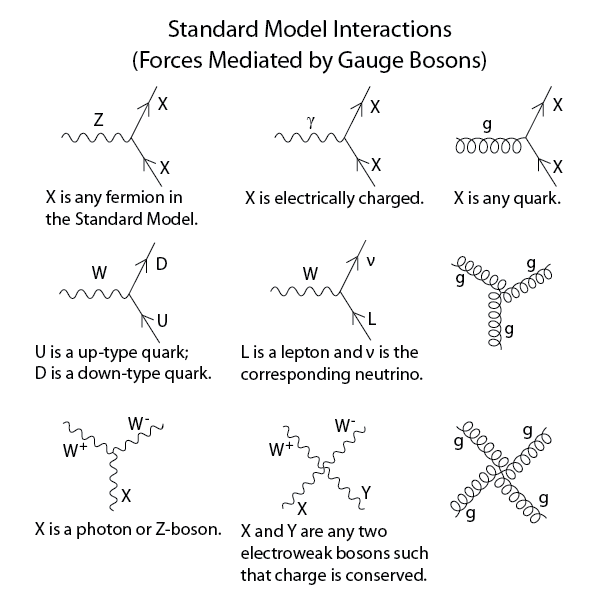
\includegraphics[width=0.6\textwidth]{/Users/rhombus/CMS/Thesis/thesis/pdfs/feyn/Standard_Model_Feynman_Diagram_Vertices.png}
    \label{fig:smcouplings}
\end{figure}
%%%%%%%%%%%%%
%%%%%%%%%%%%%
\begin{figure}[!htb]
 \center
 \caption[Feynman diagrams for $2\rightarrow2$ scattering]{
  Below are Feynman diagrams for $2\rightarrow2$ scattering. 
  These are the tree-level diagrams of the $s,t,u$
   channels respectively.
 } 
 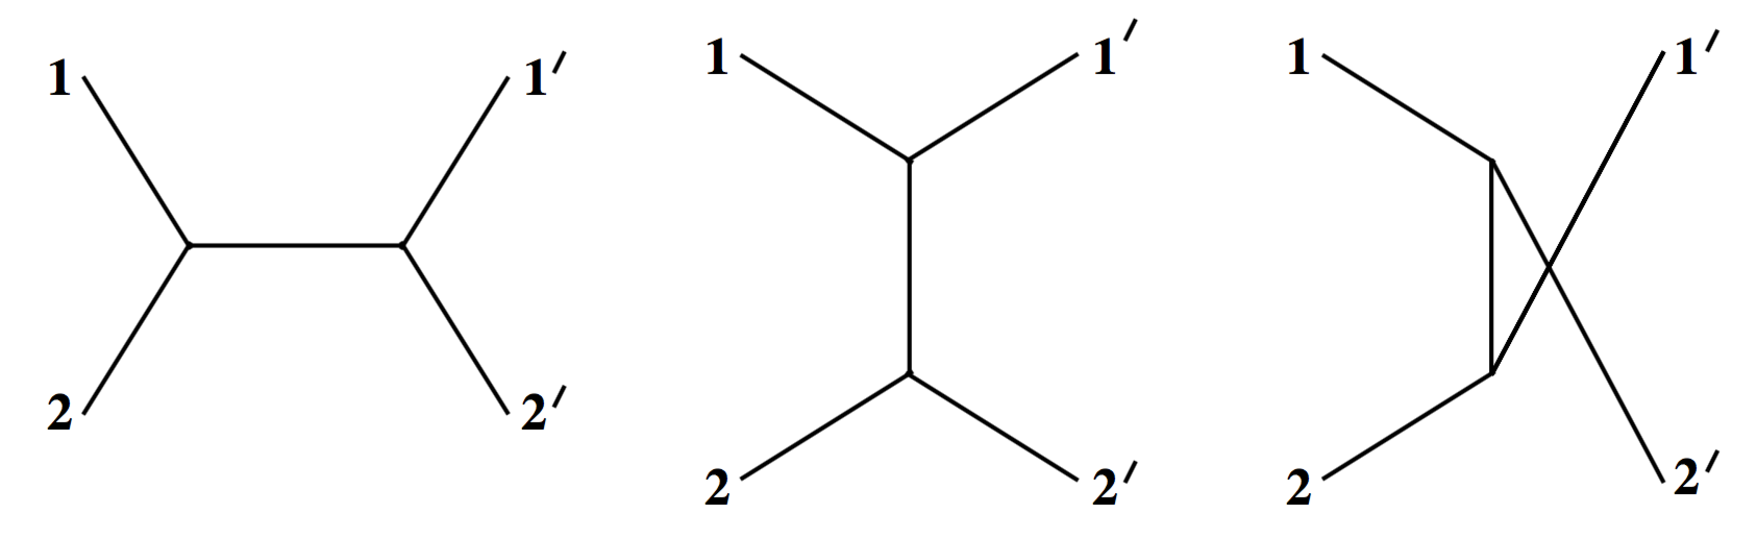
\includegraphics[width=0.6\textwidth]{/Users/rhombus/CMS/Thesis/thesis/pdfs/feyn/fenman2by2.pdf}
    \label{fig:fenyman2by2}
\end{figure}
%%%%%%%%%%%%%

\subsection{Renormalization}
 Crucial for the LSZ formulation are
  two features of quantum fields,
  that they are fully separable in the 
  infinite limit,
  $\langle 0 | \phi(x) | 0 \rangle = 0$,
  and that they are states of definite momentum,
  $ \langle k | \phi(x) | 0 \rangle = e^{-ikx}$.
 In the SM, which
  allows for fields to interact, these
  conditions are guaranteed by adjusting the
  strengths of the fundamental couplings, $g_1,g_2,g_3$.
 This ensures that the quantum states
  remain properly normalized, and is thus
  called renormalization.

 Renormalization is necessary to account
  for corrections to the tree-level propagators
  and vertices which arise from contributions
  of virtual particles connecting to 
  form closed internal loops.
 The lowest order, one-loop, diagrams
  are illustrated in Figure~\ref{fig:oneloopfeyn}.
 Renormalization is accomplished by introducing an energy scale,
  and assuming that the couplings are small compared 
  this this scale. 
 The coupling constants are therefore
  functions of energy 
  and are quoted at a particular renormalization scale,
  $\mu_R$.
 
 %% Determining if a theory is renormalizable
  % Srednicki 129, 18

 %% Consequences of running coupling constants ..

%%%%%%%%%%%%%
\begin{figure}[!tb]
 \center
 \caption[One-loop corrections to vertices and propagator]{
  Renormalization takes place via a modification
   of the coupling parameters $g_1,g_2,g_3$ to account
   for the contributions that loops of virtual
   particles make on the propagators and vertices.
  Below are diagrams keeping track of the
   flow of momentum for one-loop corrections to the 
   propagator and three and four point vertices.
 } 
 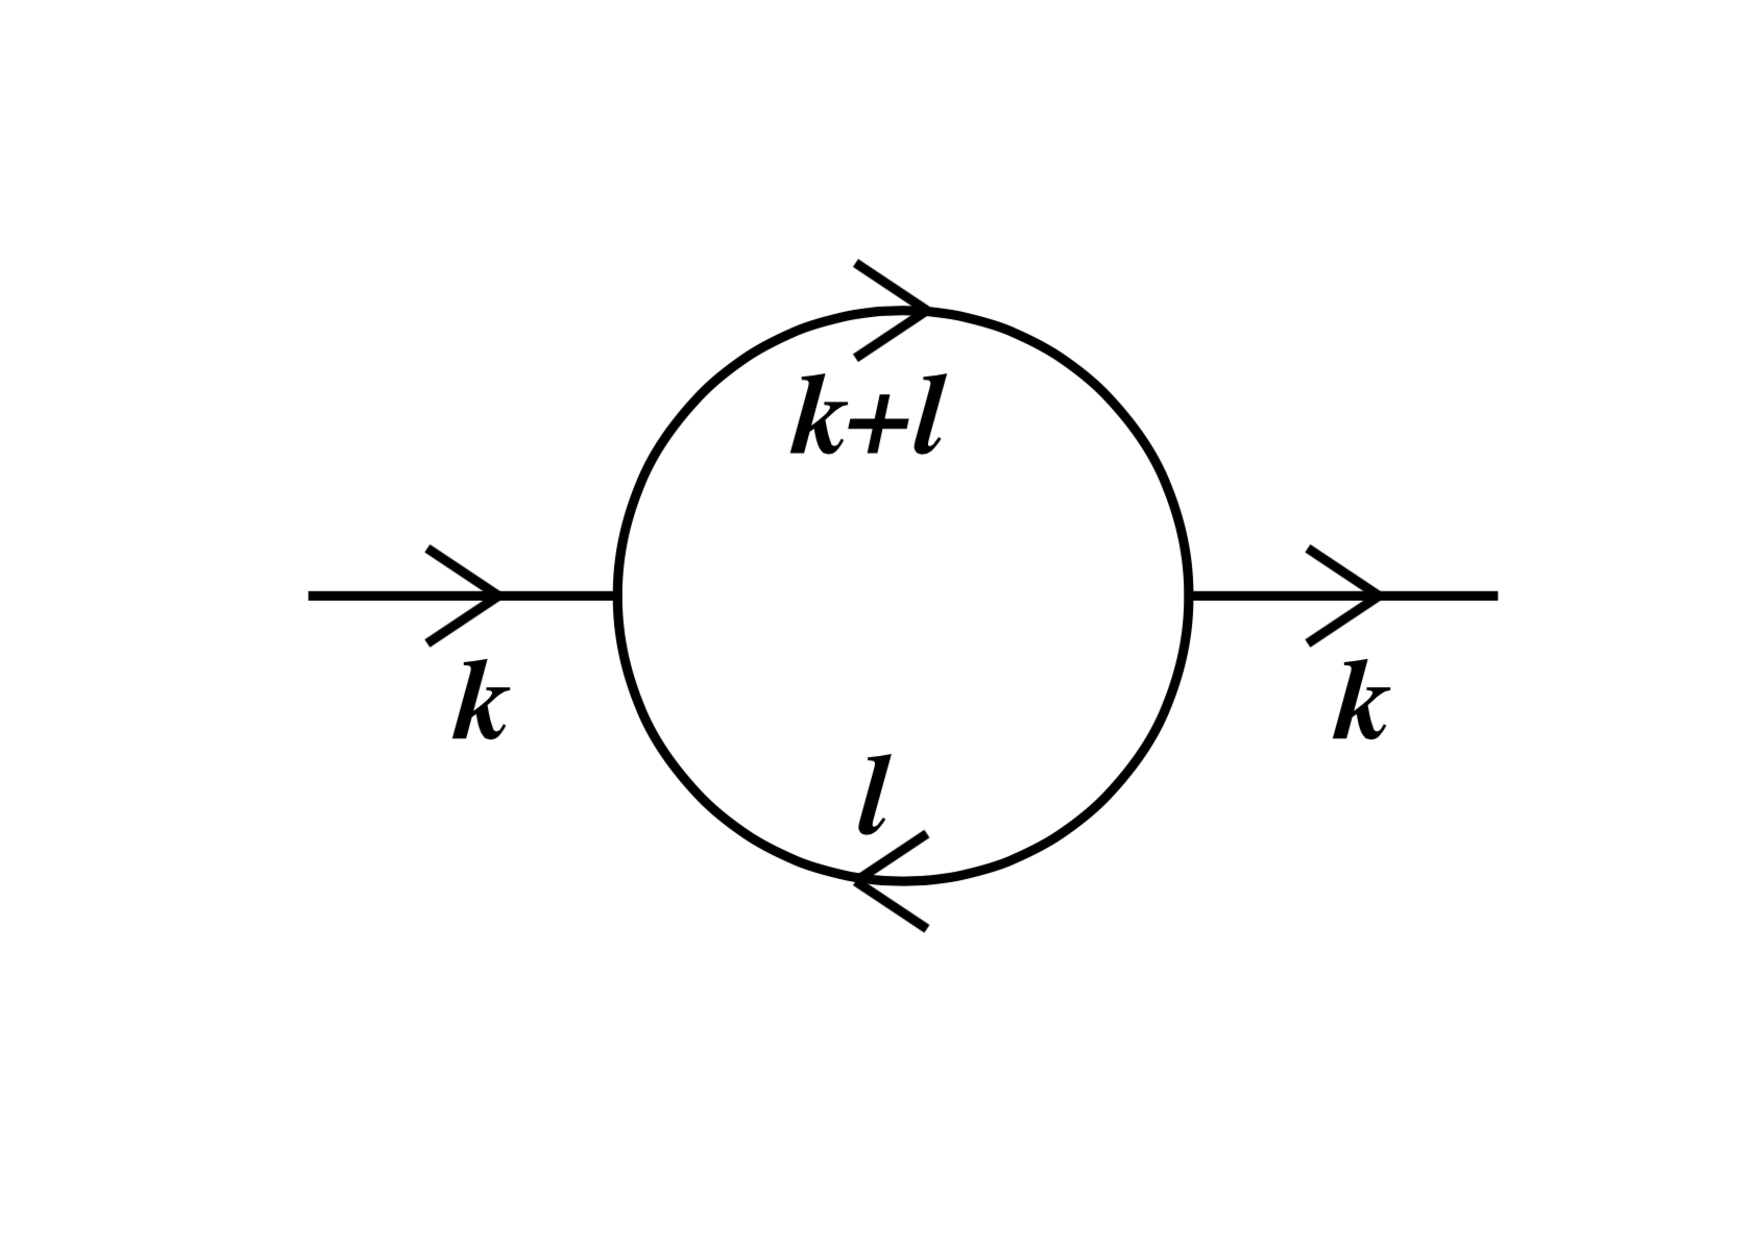
\includegraphics[width=0.3\textwidth]{/Users/rhombus/CMS/Thesis/thesis/pdfs/intro/loop_propagator.pdf}
 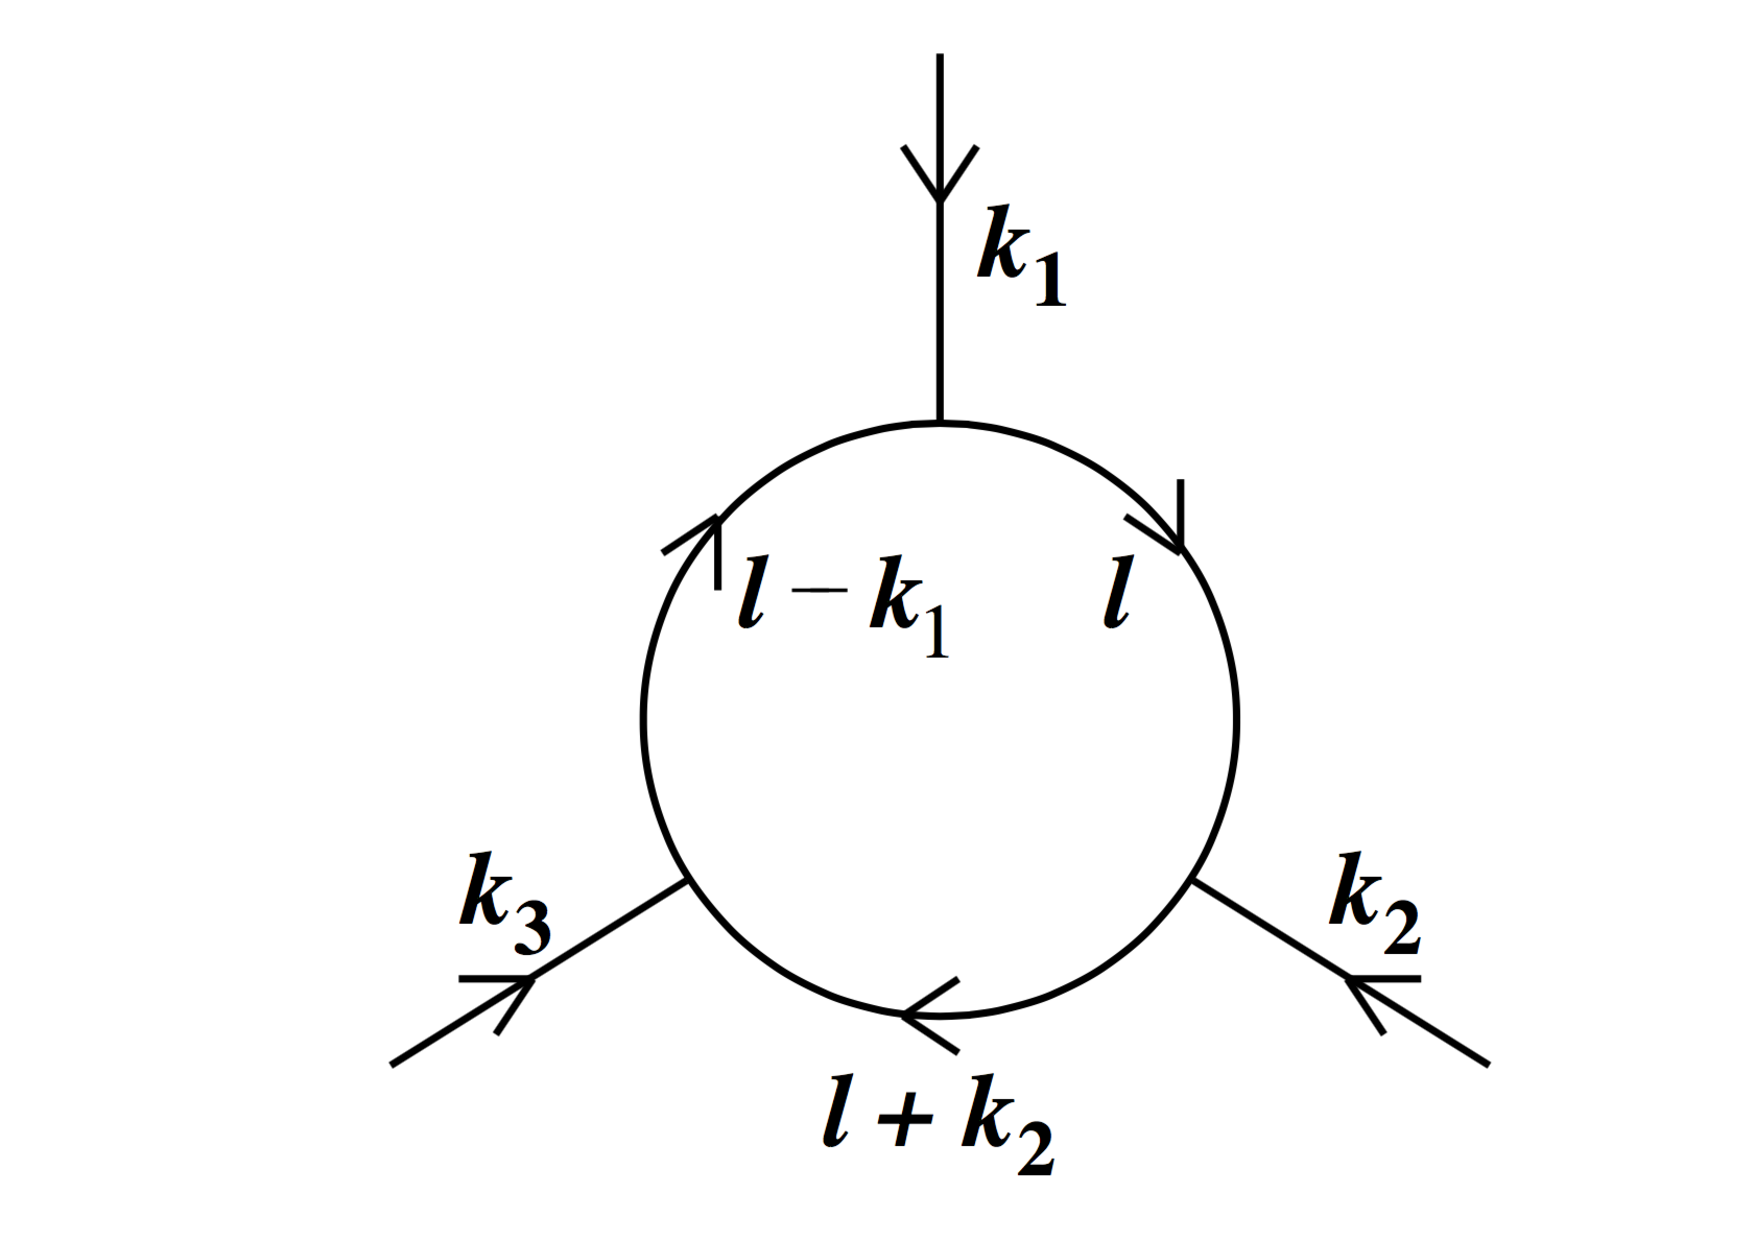
\includegraphics[width=0.3\textwidth]{/Users/rhombus/CMS/Thesis/thesis/pdfs/intro/loop_vertex.pdf}
 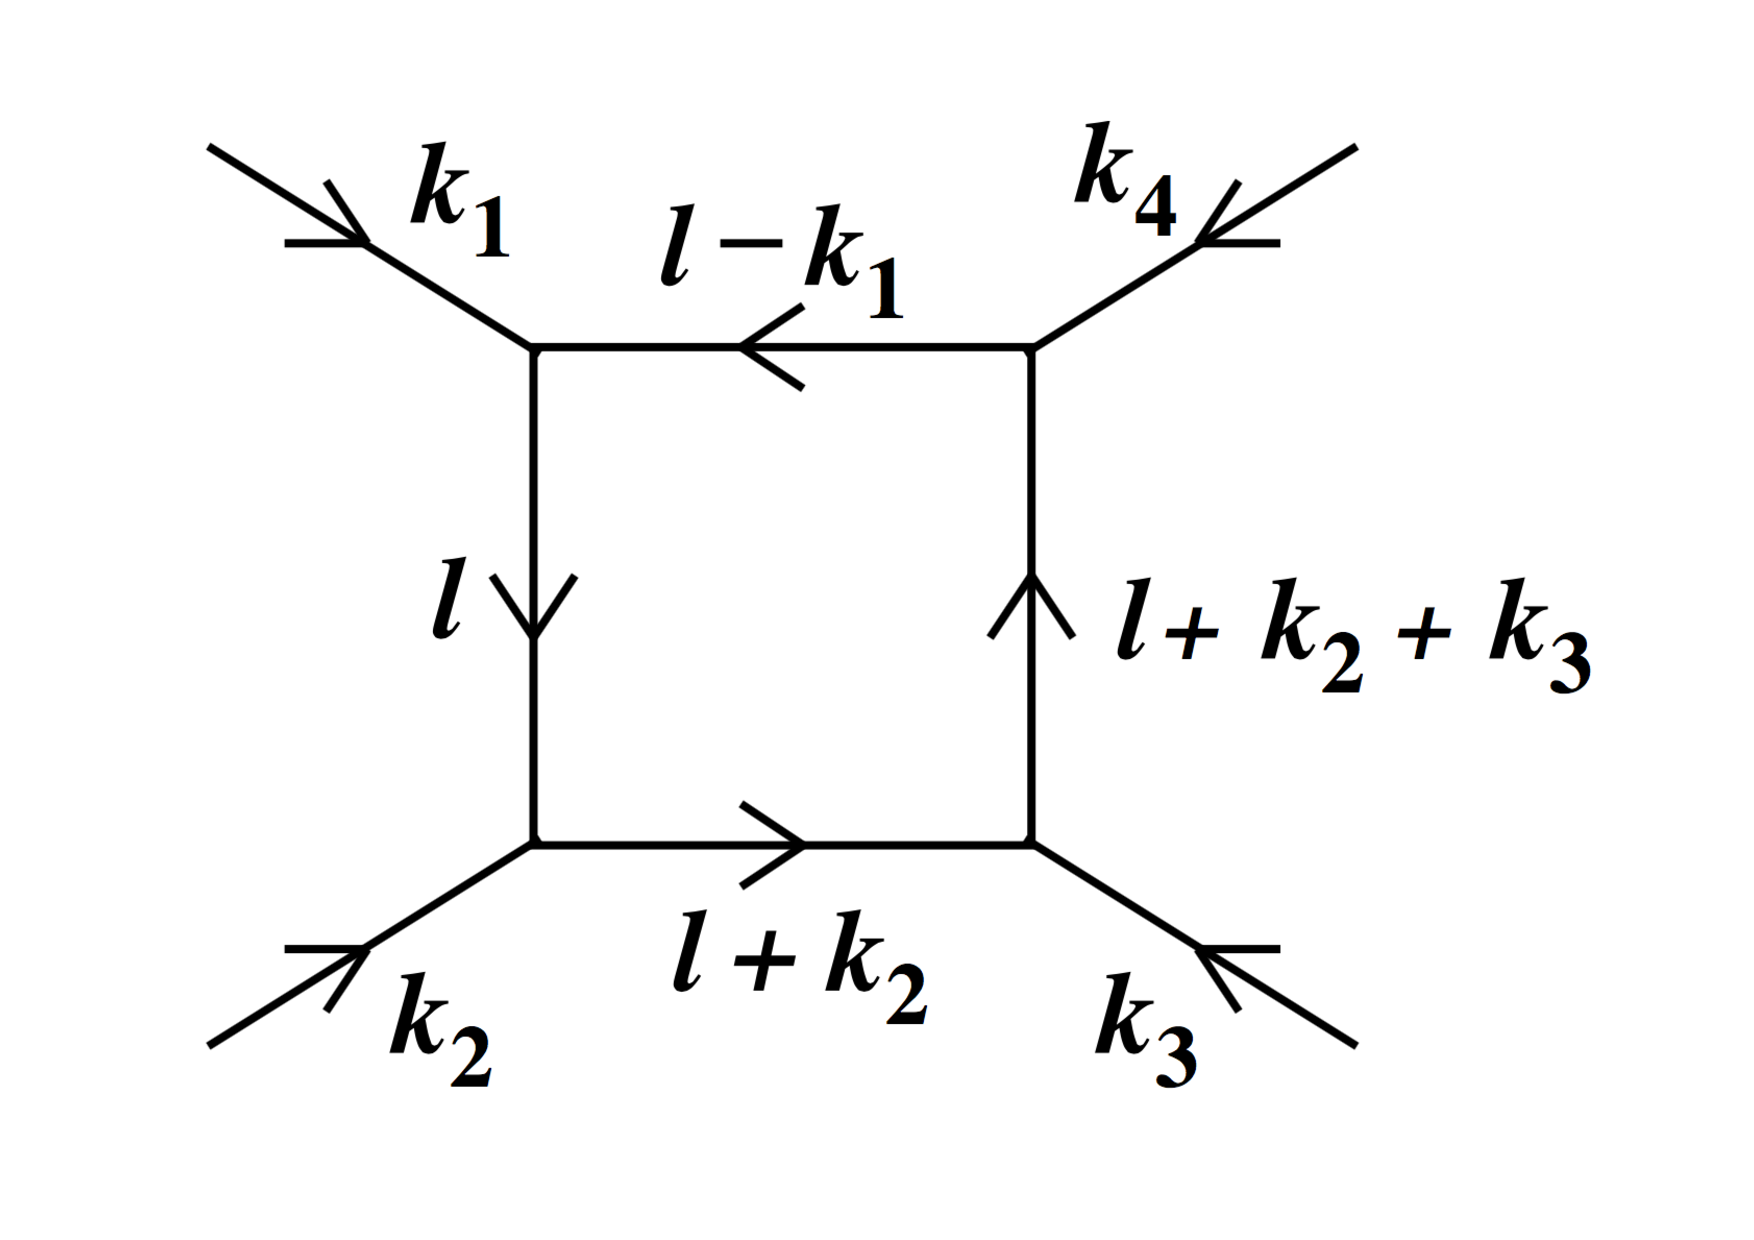
\includegraphics[width=0.3\textwidth]{/Users/rhombus/CMS/Thesis/thesis/pdfs/intro/loop_vertex4p.pdf}
    \label{fig:oneloopfeyn}
\end{figure}
%%%%%%%%%%%%%

%\subsection{Scattering amplitudes and cross sections}
\subsection{Cross sections and decay rates}

 The scattering amplitude $\langle f | i \rangle$
  is not a directly measurable observable.
 What can be observed is some finite distribution
  of data which may be analyzed to reveal
  information about the scattering amplitude.
 Quantum mechanics dictates that 
  only predictions of probability are possible,
  and the final probability of observing
  a particular interaction
  is dependent on many variables, including
  the energies, types and angular momenta of the incoming
  and outgoing particles as well as
  the masses of the propagators
  and the orientation and efficiency of the detector.

 A quantity typically measured is therefore the 
  interaction cross section, $\sigma$,
  and for the scattering of two incoming 
  particles going to $n'$ particles, $2\rightarrow n'$,
  in the CM frame, the differential is
\begin{equation}
 d\sigma = \frac{1}{4\abs{\mathbf{k}_1}_{\mathrm{CM}}}\abs{\mathcal{T}}^2 
  d\mathrm{LIPS}_{n'}(k_1 + k_2)
\end{equation}
  where the scattering matrix element, $\mathcal{T}$,
  is defined using Equation \ref{eq:lszformula}, as 
\begin{equation}\label{eq:matrixelement}
\langle f | i \rangle = (2\pi)^4\delta^4\left(\sum k_{\mathrm{in}}-\sum k_{\mathrm{out}}\right)
  i \mathcal{T}
\end{equation}
  and the Lorentz-invariant measure of the 
  phase space for the $n'$ outgoing particles is
\begin{equation}\label{eq:dlips}
 d\mathrm{LIPS}_{n'}(k) = (2\pi)^4 \delta^4
  \left(k - \sum_{j=1}^{n'}k'_i \right )
  \prod_{j=1}^{n'}dq_j'
\end{equation}
 with the Lorentz-invariant differential $dq$.

 The cross section is used to calculate the rate
  at which a process occurs, but is
  not the only relevant factor in determining
  the overall production rate.
 The production rate of a given final state
  is also dependent on the incoming
  rate of possible interactions and is 
  known as luminosity, \lumi.
 Luminosity has the units of inverse area per unit time
  and the total number of events produced
  is therefore proportional to \tlumi.
 In any real detector, final state particles
  are collected only within a finite
  solid angle and the number of particles
  scattered into a given solid angle, $\Omega$, is given by
\begin{equation}
 \frac{dN}{d\Omega} = \lumi \frac{d\sigma}{d\Omega}\;\;\;.
\end{equation}


 %The rate at which a particular event occurs
 % is proportional to \lumi and the cross section 
 % of that interaction, so it is the
 % (time) integrated luminosity that determines 
 % the total number of events produced.

 It is also possible for particles to decay
  as $1\rightarrow n'$.
 Massive particles decay to lighter ones
  in both the fermion and boson sectors,
  with all massive bosons able to 
  spontaneously decay via the diagrams in
  Figure~\ref{fig:smcouplings}.
 Of the charged fermions, only the first
  generation is stable for each type, and
  neutrinos are not known to spontaneously
  decay, but oscillate between flavors
  while propagating in free space.
 Like the differential cross section,
  the differential decay rate is a function
  of the scattering amplitude and
  has integration measure $d\mathrm{LIPS}$, 
\begin{equation}\label{eq:diffdecayrate}
 d\Gamma = \frac{1}{2E}\abs{\mathcal{T}}^2d\mathrm{LIPS}_{n'}(k)\;\;\;.
\end{equation}

 The differential decay rate is 
  inversely proportional to the energy
  of the particle, $E=\sqrt{m^2 + p^2}$.
 This means that
  comparitively heavy particles will decay
  faster than comparitively light ones
  and that energetic particles
  will appear to live longer 
  for a stationary observer due to
  relativistic time dilation effects.
 The total decay rate of a given particle
  is found by summing the decay rates from
  each of the contributing processes,
  and the primary decay channels and rates
  for the fundamental particles
  are given in Table \ref{tab:lifetimes}.

 At CMS, the heaviest quark and the heaviest
  lepton both decay before reaching
  the detector volume.
 This makes $b$ quarks the heaviest
  fundamental particles which can be seen
  to decay inside the detector,
  and therefore an object of interest.
 Additionally, their heavy mass means that they
  couple strongly with the Higgs boson
  which still has many properties that
  are under investigation.
 The $W$ and $Z$ bosons are both so 
  massive that they decay before reaching
  the innermost layers of the detector
  and are often identified by their decay products
  pointing back to a common vertex.
 
%%%% Table SU(2) Representations
\begin{table}[tb]
\caption[Fundamental particle decay channels and rates]
{
 Below are listed the decay channels and 
  rates for each of the unstable
  fundamental particles.
 At CMS, with the detection apparatus
  located a finite distance away from the
  interaction vertex, particles such as the
  $W$, $Z$ and Higgs bosons,
  as well as the $t$ and $tau$, decay before
  reaching the first layer of the detector.
}
\label{tab:lifetimes}
\begin{center}
\resizebox{\columnwidth}{!}{
\begin{tabular}{r|l|l|l}
Particle & Primary decay modes(s) & Total rest-frame $d\Gamma$ & Typical decay location \\
\hline\hline
$W$ & $W\rightarrow \ell\nu$ & X & Before reaching CMS \\
$Z$ & $Z\rightarrow f\overline{f}$ (for $2M_f < M_Z$) & X & Before reaching CMS \\
$\tau$ & $\tau\rightarrow W \nu_\tau$ & X & Before reaching CMS \\
$\mu$  & $\mu\rightarrow W \nu_\mu$ & X & After leaving CMS \\
$t$    & $t\rightarrow Wb$ & X & Before reaching CMS \\
$b$    & $b\rightarrow Wc$ & X & Inside CMS \\
$c$    & $c\rightarrow Ws$ & X & Inside CMS \\
$s$    & $s\rightarrow Wu$ & X & Inside CMS
\end{tabular}
}
\end{center}
\end{table}
%%%%%%%
 





% For initial and final states
%  of quantum fields, 
% $|i\rangle$ and $f\rangle$, the 
% amplitude of the overlap between states is a function of 
% the scattering amplitude $\mathcal{M}$ and 
% subject to momentum conservation,
%\begin{equation}\label{eq:fidirac}
% \left | \langle f | i \rangle \right |^2 = A
%  \left ( \delta^4 ( k_{\mathrm{in}} - k_{\mathrm{out}} ) \right )\left |\mathcal{M}\right |^2\;\;\;.
%\end{equation}
 
%%
%%% The photon only couples to charged particles, 
%%%  and does so .
%%% If kinematically allowed, a gluon is able to
%%%  split into a quark-antiquark pair and 
%%%  $W$ bosons can decay into lepton-neutrino pairs
%%%  with the lepton and the neutrino belonging to the same
%%%  type.
%%% The $Z$ boson can decay into any fermion-antifermion
%%%  pair, but charge must be conserved in such an interaction
%%%  and interactions involving fermions and neutral 
%%%  bosons must remain within a given generation.
%%
%%
\subsection{QCD and Proton Structure}
 The Feynman diagrams introduced in Section \ref{sec:PIandFD}
  describe the interactions between fundamental particles,
  but at the LHC, collisions take place between
  protons, which are composit.

 One feature of the $SU(3)$ symmetry of the
  strong force is that gluons
  carry one unit of color and one unit of anticolor
  while the quarks carry one unit of color charge.
 This is what allows gluons to interact with each other
  as well as with quarks.
 That quark confinement is necessitated by the $SU(3)$
  structure has not been conclusively determined, 
  but observationally, a free gluon or quark has 
  never been observed.
 Instead, quarks appear as bound in colorless (singlet)
  combinations called hadrons
  which are further classified as mesons ($q\overline{q}$)
  or as baryons ($qqq$ or
  $\overline{q}\overline{q}\overline{q}$),
  and are held together by gluons.
 Evidently, the binding energy of the
  quarks has a form such that
  after a distance of roughly $10^{-15}$ meters,
  the energy
  stored in the gluon field is greater
  than the energy needed to create a
  quark-antiquark pair, bringing the pair
  into existance.
 This process of energetic quarks
  creating particles as they
  separate is called hadronization
  and is an important effect at the LHC.

 Protons are a type of baryon and
  at low energy, may combine with a single electron 
  to form a neutral hydrogen atom.
 At higher energies, the internal structure 
  of the proton becomes more evident,
  and it contains three valence quarks, $uud$, 
  which are constantly exchanging gluons.
 When probed at high enough energy, or equivalently,
  at short enough length scales, these 
  gluons can also each split into a $q\overline{q}$ pair 
  which typically reannihialate with each other.
 With gluons inside the proton splitting into quarks
  and coupling with other gluons,
  this forms a `sea' of quarks and gluons,
  and as protons are acceleratded
  to energies of \GeV or \TeV as is the case at the
  LHC, the fraction of the momentum of the
  proton attributed to the gluons becomes higher 
  than that attributed to the valence quarks.

 A proton-proton collider was therefore a 
  sensible choice for the LHC. 
 The physics goals of the project are
  to measure quantities associated with a wide range SM 
  processes and to continue the search for 
  evidence of new physics.
 Quarks interact with all of the gauge bosons
  as well as with the Higgs boson
  and the proton contains the two lightest
  quarks of each type
  in addition to the gluons and sea.
 Colliding proton beams thus allow for
  the interactions between many different
  initial particle configurations to be explored,
  and with the exception of the neutrinos which 
  interact only via the weak exchange of the $Z$
  boson and escape the detectors,
  all other fundamental SM particles have been
  directly  observed  at CERN. 

%%%\section{Beyond the Standard Model}
%%% Here we describe ways to extend the Standard Model, including need for extensions: dark matter
%%
